\section{Durchführung}
\label{sec:Durchführung}

Der prinzipielle Versuchsaufbau ist in Abbildung \ref{fig:aufbau} dargestellt. Die Alphastrahlung aus der 241-Americium-Quelle wird kollimiert. Die darauffolgende Folie kann ein- oder ausgebaut werden, um auch Studien der Reichweite von Alphastrahlung in Luft ohne Target durchzuführen. Der auf einer Schiene bewegliche Detektor ist ein Surface-Barrier-Detektor, der im Grunde einer Diode in Sperrrichtung entspricht.
In einem p-n-Übergang bildet sich eine Verarmungszone, in der durch einfallende Strahlung Elektronen-Loch-Paare entstehen. Diese werden durch das vorherrschende elektrische Feld, das durch die Sperrspannung hervorgerufen wird, zu den Elektroden hin abgesaugt und erzeugen einen messbaren elektrischen Impuls, der durch einen Verstärker noch weiter verstärkt werden kann.

\begin{figure}
  \centering
  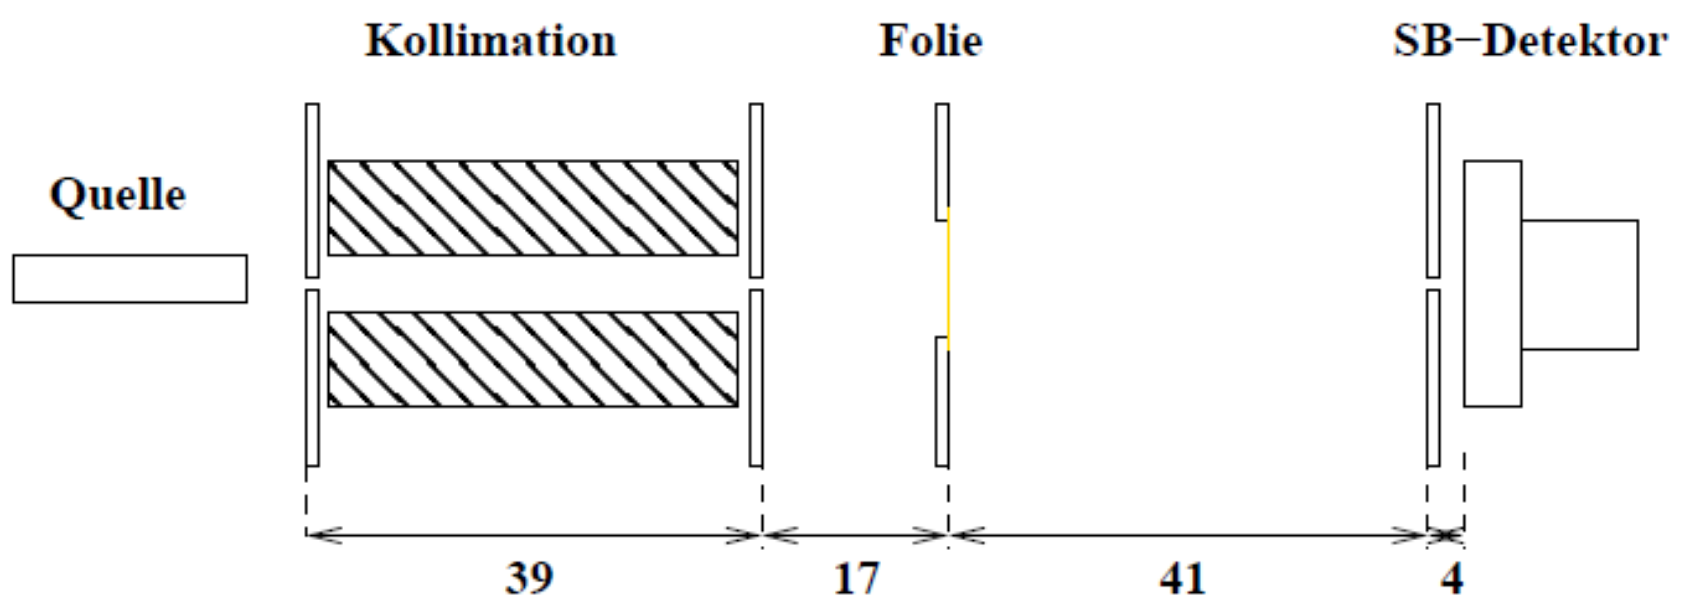
\includegraphics[width=\textwidth]{images/aufbau.png}
  \caption{Schematische Darstellung des Versuchsaufbaus mit seinen Abmessungen \cite{Versuchsanleitung}.}
  \label{fig:aufbau}
\end{figure}

Der Aufbau kann durch eine sogenannte Drehschieberpumpe evakuiert werden, um die Energieverluste der $\alpha$-Strahlung als Funktion des Drucks in der Kammer zu studieren. Der Aufbau einer Drehschieberpumpe ist in Abbildung \ref{fig:pumpe} dargestellt.
Die Pumpe besteht aus zwei Zylindern, wobei der innere Zylinder asymmetrisch im äußeren Zylinder die Wand berührend eingelassen ist. Er berührt die Außenwand zwischen der Ein- und Auslassöffnung und rotiert. An ihm sind Drehschieber angebracht, die rotieren und dadurch abgetrennte Bereiche bilden. Während der Rotation verringert sich die Größe eines dieser Räume, sodass das zuvor eingesaugte Gas komprimiert wird und an der Auslassöffnung ausgestoßen wird.

\begin{figure}
  \centering
  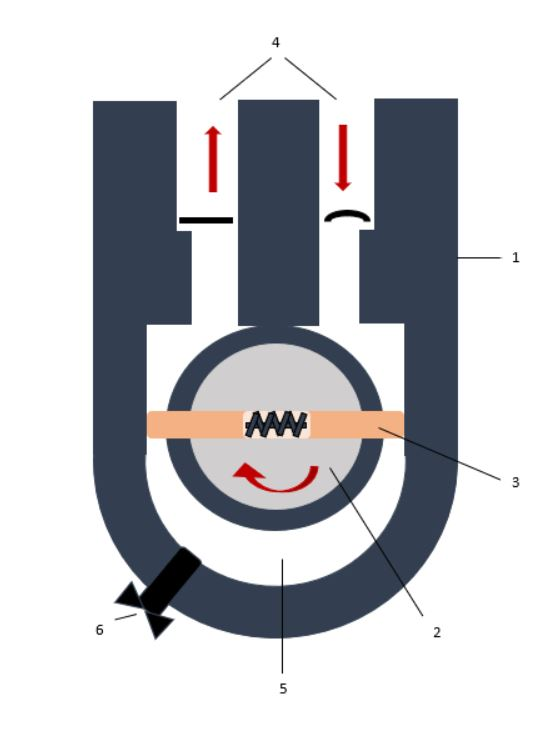
\includegraphics[width=\textwidth]{images/pumpe.jpg}
  \caption{Schematische Darstellung einer Drehschieberpumpe. Der innere Zylinder (2) rotiert nicht-zentral in dem Gehäuse (1). Der Drehschieber (3) rotiert und bildet abgetrennte Bereiche (z.B. (5)). Die Ein- und Auslassöffnungen (4) befinden sich am oberen Rand des Gehäuses, während unten ein Gasballast (6) durch Luftzufuhr die Kondensatbildung verhindert. \cite{pumpe}}
  \label{fig:pumpe}
\end{figure}
